\documentclass[aps,prb,twocolumn,superscriptaddress,floatfix,longbibliography]{revtex4-2}

\usepackage[utf8]{inputenc}
\usepackage[spanish]{babel}
\usepackage{graphicx}
\usepackage{amsmath}
\usepackage{subcaption}
\usepackage{wrapfig} 
\usepackage[export]{adjustbox}

\usepackage{amsmath,amssymb} % math symbols
\usepackage{bm} % bold math font
\usepackage{graphicx} % for figures
\usepackage{comment} % allows block comments
\usepackage{textcomp} % This package is just to give the text quote '
\usepackage{listings} %para agregar código

%\usepackage{ulem} % allows strikeout text, e.g. \sout{text}

\usepackage[spanish]{babel}

\usepackage{enumitem}
\setlist{noitemsep,leftmargin=*,topsep=0pt,parsep=0pt}

\usepackage{xcolor} % \textcolor{red}{text} will be red for notes
\definecolor{lightgray}{gray}{0.6}
\definecolor{medgray}{gray}{0.4}

\usepackage{hyperref}
\hypersetup{
colorlinks=true,
urlcolor= blue,
citecolor=blue,
linkcolor= blue,
bookmarks=true,
bookmarksopen=false,
}

% Code to add paragraph numbers and titles
\newif\ifptitle
\newif\ifpnumber
\newcounter{para}
\newcommand\ptitle[1]{\par\refstepcounter{para}
{\ifpnumber{\noindent\textcolor{lightgray}{\textbf{\thepara}}\indent}\fi}
{\ifptitle{\textbf{[{#1}]}}\fi}}
%\ptitletrue  % comment this line to hide paragraph titles
%\pnumbertrue  % comment this line to hide paragraph numbers

% minimum font size for figures
\newcommand{\minfont}{6}

% Uncomment this line if you prefer your vectors to appear as bold letters.
% By default they will appear with arrows over them.
% \renewcommand{\vec}[1]{\bm{#1}}

%Cambiar Cuadros por Tablas y lista de...
%\renewcommand{\listtablename}{Índice de tablas}
\renewcommand{\tablename}{Tabla}
\renewcommand{\date}{Fecha}

% \graphicspath{ {C:/Users/lupam/Mi unidad/Pablo Chehade/Instituto Balseiro (IB)/Laboratorio Avanzado/Informe/V5/Figures} } %Para importar imagenes desde una carpeta


\lstset{
  basicstyle=\ttfamily\small,
  breaklines=true,
  frame=single,
  numbers=left,
  numberstyle=\tiny,
  keywordstyle=\color{blue},
  commentstyle=\color{green},
  stringstyle=\color{red},
} %Configuración para el bloque de código


\usepackage[bottom]{footmisc} %para que las notas al pie aparezcan en la misma página



\begin{comment}

%Comandos de interes:

* Para ordenar el documento:
\section{Introducción}
\section{\label{sec:Formatting}Formatting} %label para luego hacer referencia a esa sección

\ptitle{Start writing while you experiment} %pone nombre y título al documento dependiendo de si en el header están los comandos \ptitletrue y \pnumbertrue

* Ecuaciones:
\begin{equation}
a^2+b^2=c^2 \,.
\label{eqn:Pythagoras}
\end{equation}

* Conjunto de ecuaciones:
\begin{eqnarray}
\label{eqn:diagonal}
\nonumber d & = & \sqrt{a^2 + b^2 + c^2} \\
& = & \sqrt{3^2+4^2+12^2} = 13
\end{eqnarray}

* Para hacer items / enumerar:
\begin{enumerate}
  \item
\end{enumerate}

\begin{itemize}
  \item
\end{itemize}

* Figuras:
\begin{figure}[h]
    \includegraphics[clip=true,width=\columnwidth]{pixel-compare}
    \caption{}
     \label{fig:pixels}
\end{figure}

* Conjunto de figuras:
(no recuerdo)


* Para hacer referencias a fórmulas, tablas, secciones, ... dentro del documento:
\ref{tab:spacing}

* Para citar
Elementos de .bib
\cite{WhitesidesAdvMat2004}
url
\url{http://www.mendeley.com/}\\

* Agradecimientos:
\begin{acknowledgments}
We acknowledge advice from Jessie Zhang and Harry Pirie to produce Fig.\ \ref{fig:pixels}.
\end{acknowledgments}

* Apéndice:
\appendix
\section{\label{app:Mendeley}Mendeley}

* Bibliografía:
\bibliography{Hoffman-example-paper}

\end{comment}


\begin{document}

% Allows to rewrite the same title in the supplement
\newcommand{\mytitle}{Aprendizaje no supervisado}

\title{\mytitle}

\author{Pablo Chehade \\
    \small \textit{pablo.chehade@ib.edu.ar} \\
    \small \textit{Redes Neuronales, Instituto Balseiro, CNEA-UNCuyo, Bariloche, Argentina, 2023} \\}
    
\maketitle




\section*{Ejercicio 1}


Se entrenó de manera no supervisada una red neuronal lineal de una sola capa con cuatro entradas y una salida. Los datos de entrada presentan una distribución gaussiana con matriz de correlación $\Sigma$



\[
\Sigma = \begin{bmatrix}
2 & 1 & 1 & 1 \\
1 & 2 & 1 & 1 \\
1 & 1 & 2 & 1 \\
1 & 1 & 1 & 2 \\
\end{bmatrix}
.
\]
El autovector asociado al mayor autovalor de $\Sigma$ es $\vec{v} = \frac{1}{2}(1, 1, 1, 1)$. 


Se partió de un vector de pesos $\vec{w} = (w_1, w_2, w_3, w_4)$, con cada componente dada por una distribución uniforme con máximo $0.01$. Luego, se aplicó la regla de Oja
\[
\Delta w_j = \eta V ( \xi_j - V w_j ).
\]
Aquí, $\eta$ representa la tasa de aprendizaje, $V$ es la salida de la red y $\xi_j$ es la componente $j$ del dato de entrada $\vec{\xi}$. En base a la teoría desarrollada para la regla de Oja, se espera que el vector de pesos $\vec{w}$ tienda al autovector $\vec{v}$.


En la figura \ref{fig:ej1_fig1}, se ilustra la evolución del módulo de los pesos $|w_j|$, las modificaciones $\Delta w_j$ y la diferencia entre $w_j$ y $v_j$, para $\eta = 0.001$. Tras un período transitorio, se observa que las componentes de $\vec{w}$ tienden hacia el valor $0.5$, indicando convergencia hacia $\vec{v}$. Dependiendo de las condiciones iniciales, el vector $\vec{w}$ tiende a alinearse en la dirección $+\vec{v}$ o $-\vec{v}$. Debido a esto se graficó el módulo de cada componente. Posteriormente, en estado estacionario, los pesos continúan modificándose. Por ello, en la figura \ref{fig:ej1_fig2}, se procesan los datos anteriores realizando un promedio en cada paso de tiempo de los 200 pasos adyacentes. Esto resulta en un comportamiento más suave y una reducción notable en las variaciones de $\Delta w_j$ de hasta un orden de magnitud. Luego de este procesamiento de los datos se confirma nuevamente que $\vec{w}$ tiende a $\vec{v}$.

Por último, en la figura \ref{fig:ej1_fig3}, se evolucionó el sistema con $\eta = 0.01$. El sistema muestra una convergencia más rápida y variaciones $\Delta w_j$ de mayor magnitud. Además, se determinó que existe un valor superior límite para $\eta$, más allá del cual el sistema tiende a diverger.

\section*{Ejercicio 2}

Se entrenó una red neuronal de Kohonen con dos neuronas de entrada y diez neuronas de salida alineadas en una línea. La red se alimenta mediante una distribución de entrada definida como:

\[ P(\xi) = P(r, \theta) = 
  \begin{cases} 
   \text{constante} & \text{si } r \in [0.9, 1.1], \, \theta \in [0, \pi] \\
   0 & \text{si no},
  \end{cases} \]
donde $r$ y $\theta$ son las coordenadas polares del vector $\vec{\xi}$.

Los pesos iniciales \(w_{ij}\), donde \(i\) representa la neurona de salida y \(j\) la dimensión del espacio de entrada, se asignan aleatoriamente con una distribución uniforme con un valor máximo de 0.1. En cada iteración del entrenamiento, se selecciona un vector de entrada \(\vec{\xi}\), y se identifica la neurona "ganadora" \(i^*\) como aquella que minimiza la distancia euclidiana con el vector de entrada, es decir

\[ i^* = \text{argmin}_i |\vec{w}_i - \vec{\xi}|, \]
donde $\vec{w}_i = (w_{i1}, w_{i2})$. Posteriormente, se actualizan los pesos de todas las neuronas utilizando la regla
\[ \Delta \vec{w}_i = \eta \, \Gamma(i, i^*) \, (\vec{\xi} - \vec{w}_i), \]
donde 
\[ \Gamma(i, i^*) = \exp\left( - \frac{(i - i^*)^2}{2 \sigma^2} \right) \]
es la función de vecindad y \(\eta\) es la tasa de aprendizaje.

Se realizó un análisis sobre la evolución de los pesos de la red variando los parámetros \(\eta\) y \(\sigma\), y se observó cómo afectan la convergencia, haciendo incapié cómo se modifican los pesos durante el entrenamiento.

Se observaron diferentes comportamientos al variar los parámetros \(\eta\) y \(\sigma\). En todos los casos se estudió la convergencia de los pesos $\vec{w}_i$ mediante su evolución graficada en el espacio de los datos de entrada (figura \ref{fig:ej2_fig1})

\begin{enumerate}
    \item \(\eta = 0.1\) y \(\sigma = 1\): Inicialmente los pesos \(\vec{w}_i\) son cercanos entre sí. Luego se desplazan hacia las regiones donde \(P(\vec{\xi})\) es no nula. Finalmente, los pesos se organizan sobre la región, organizados de acuerdo a la disposición de las neuronas sobre la línea.

    \item \(\eta = 0.1\) y \(\sigma = 2\): En este caso, los pesos se mueven más juntos en comparación con el caso anterior debido a un mayor valor de \(\sigma\), que incrementa el efecto de la función de vecindad. Esto se puede entender más claramente en el caso extremo en el que $\sigma \rightarrow \infty$. En tal caso, $\Gamma \rightarrow 1$ y todas las neuronas se actualizan en la misma magnitud hacia la posición del dato de entrada $\vec{\xi}$. En cuanto al estado final, incluso con una gran cantidad de pasos de entrenamiento no se llega al mismo estado que antes. Una forma de resolver este problema podría ser aprovechando el comportamiento visto en el caso anterior y disminuir progresivamente $\sigma$ a medida que se realiza el entrenamiento.
    

    \item \(\eta = 0.01\) y \(\sigma = 1\): Con una tasa de aprendizaje reducida, la evolución es más lenta. Además, los pesos muestran variaciones menores durante el entrenamiento. A pesar de la lentitud, con suficientes iteraciones el sistema converge a la misma condición que el primer caso.

\end{enumerate}

El estudio sugiere que la elección de \(\eta\) y \(\sigma\) es crucial. Un \(\eta\) más bajo lleva a una convergencia más lenta pero con menor ruido, mientras que un \(\sigma\) más alto promueve una adaptación global pero menos detallada de los pesos. 


\onecolumngrid



\begin{figure}
  \centering
  \begin{subfigure}[b]{0.3\textwidth}
      \centering
      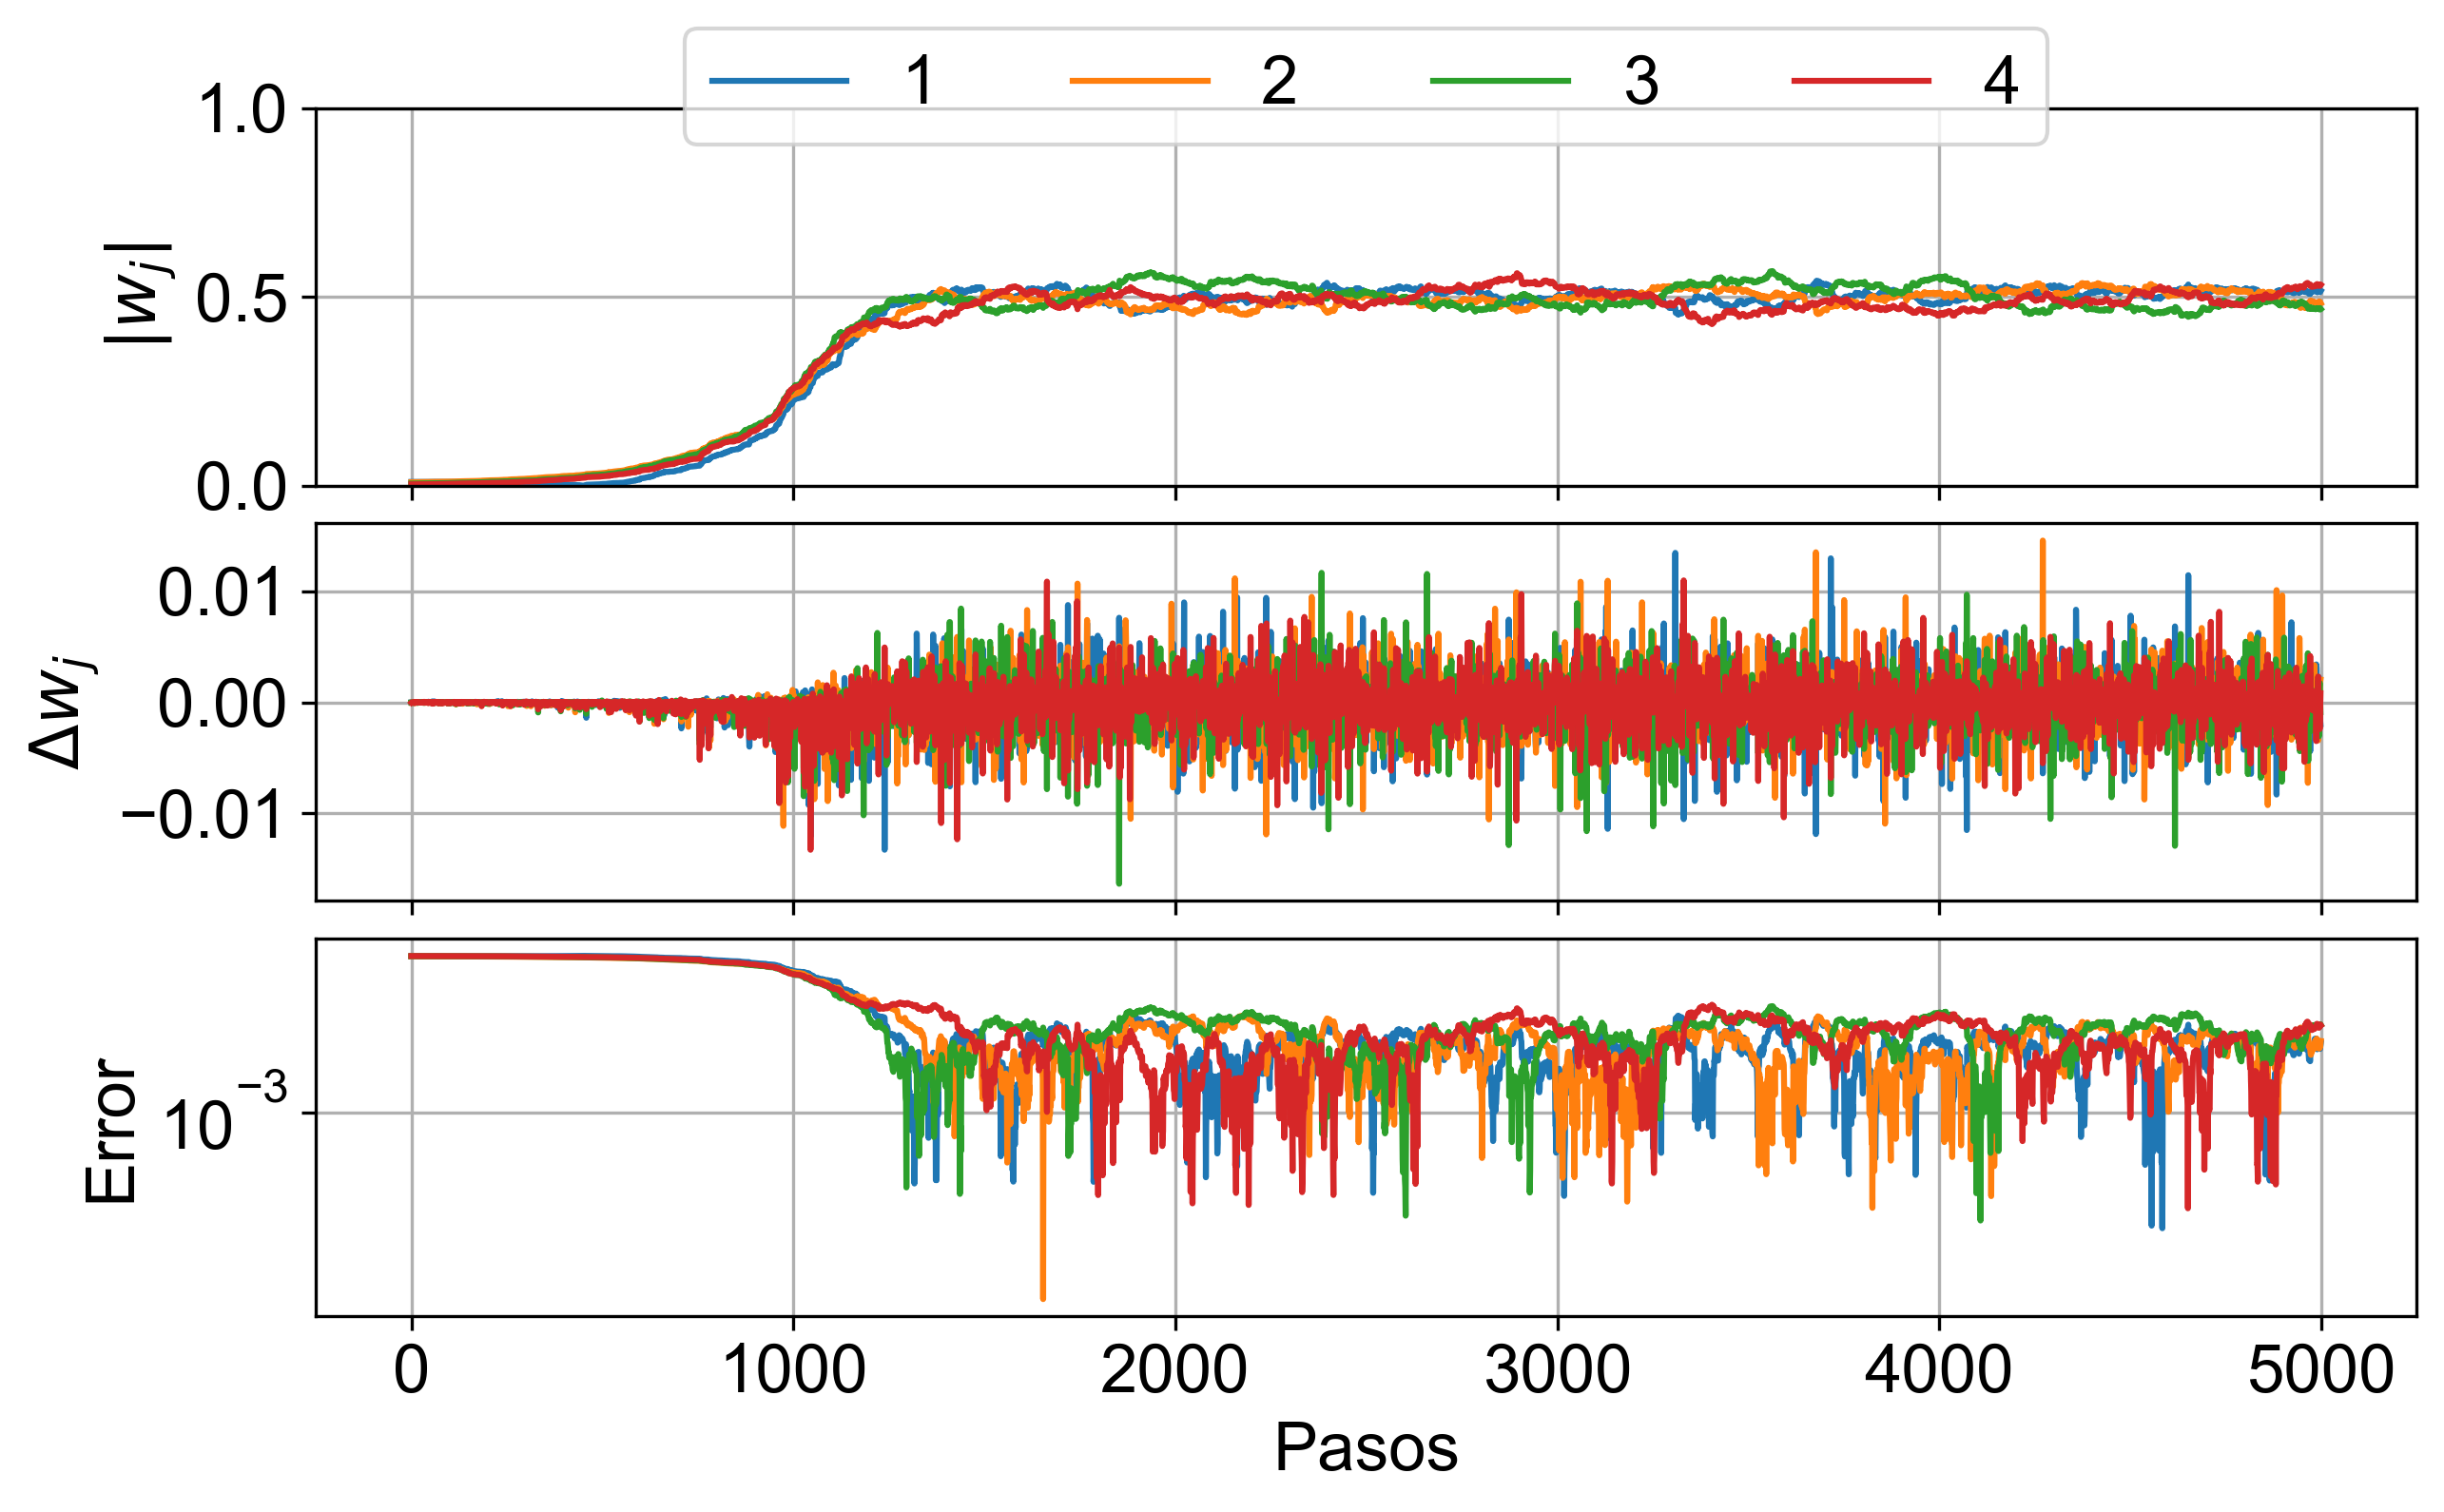
\includegraphics[width=\textwidth]{ej1_fig1.png}
      \caption{\label{fig:ej1_fig1}}
  \end{subfigure}
  \hfill
  \begin{subfigure}[b]{0.3\textwidth}
      \centering
      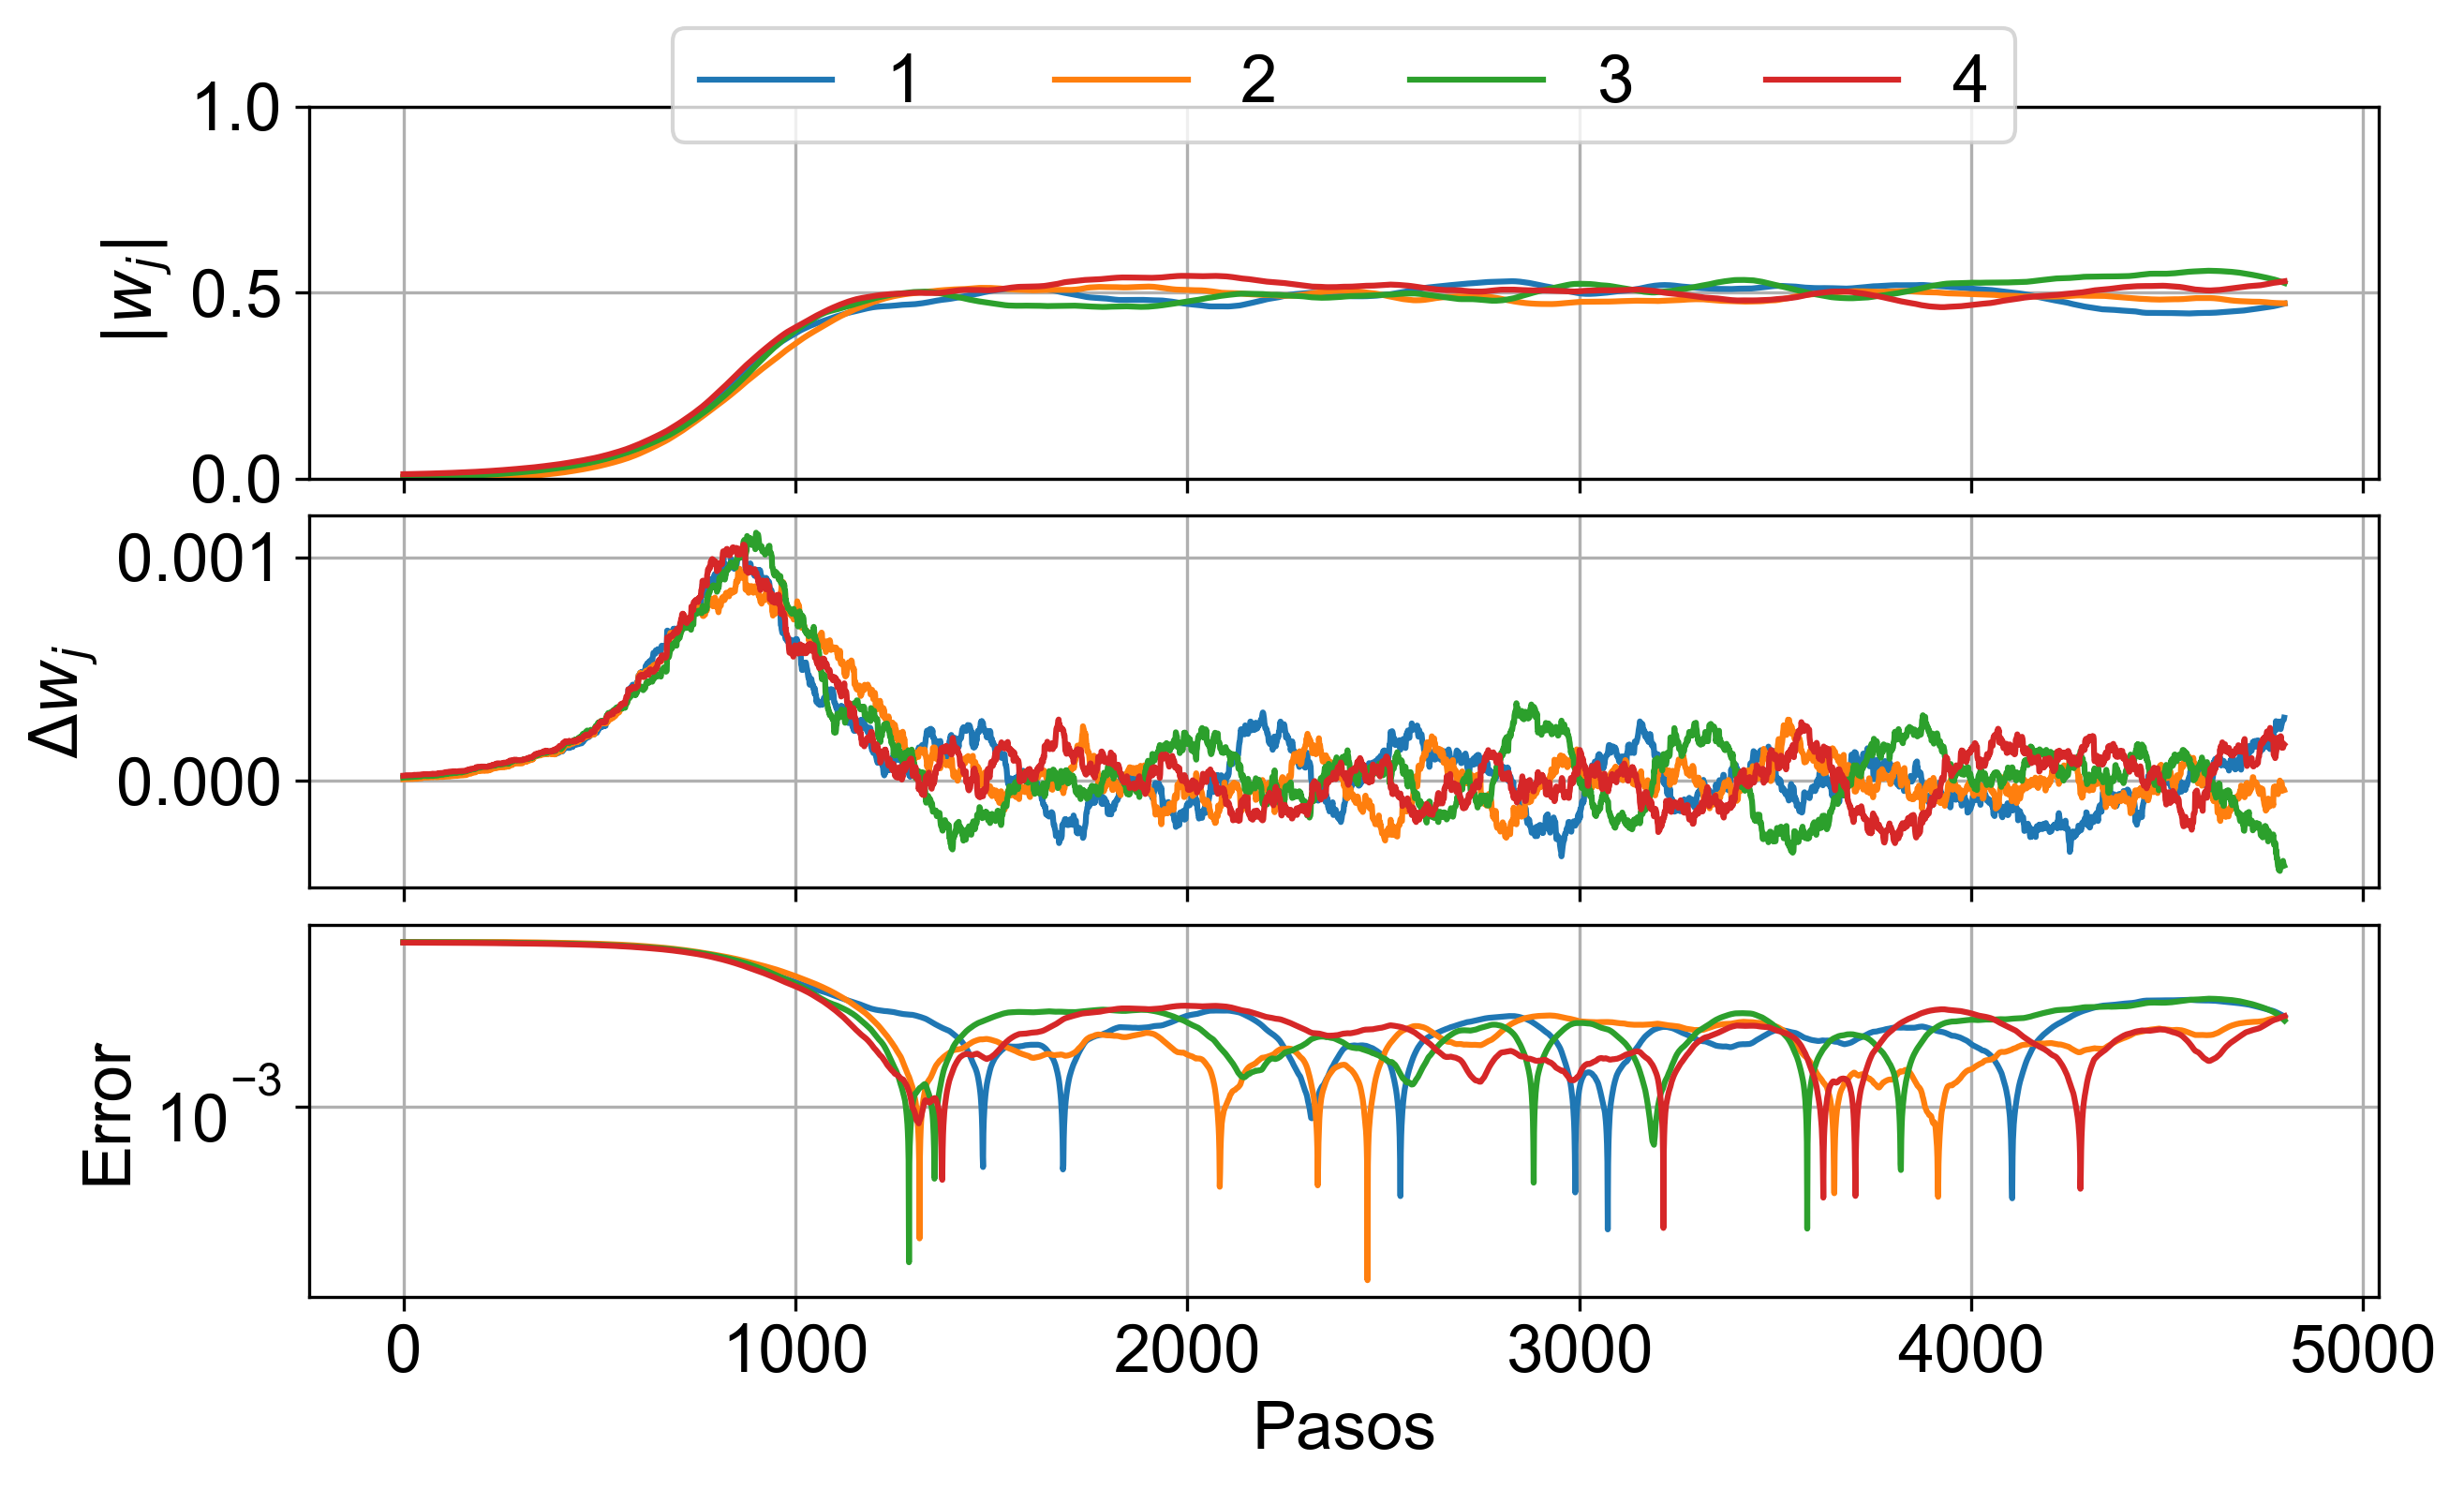
\includegraphics[width=\textwidth]{ej1_fig2.png}
      \caption{\label{fig:ej1_fig2}}
  \end{subfigure}
  \hfill
  \begin{subfigure}[b]{0.3\textwidth}
      \centering
      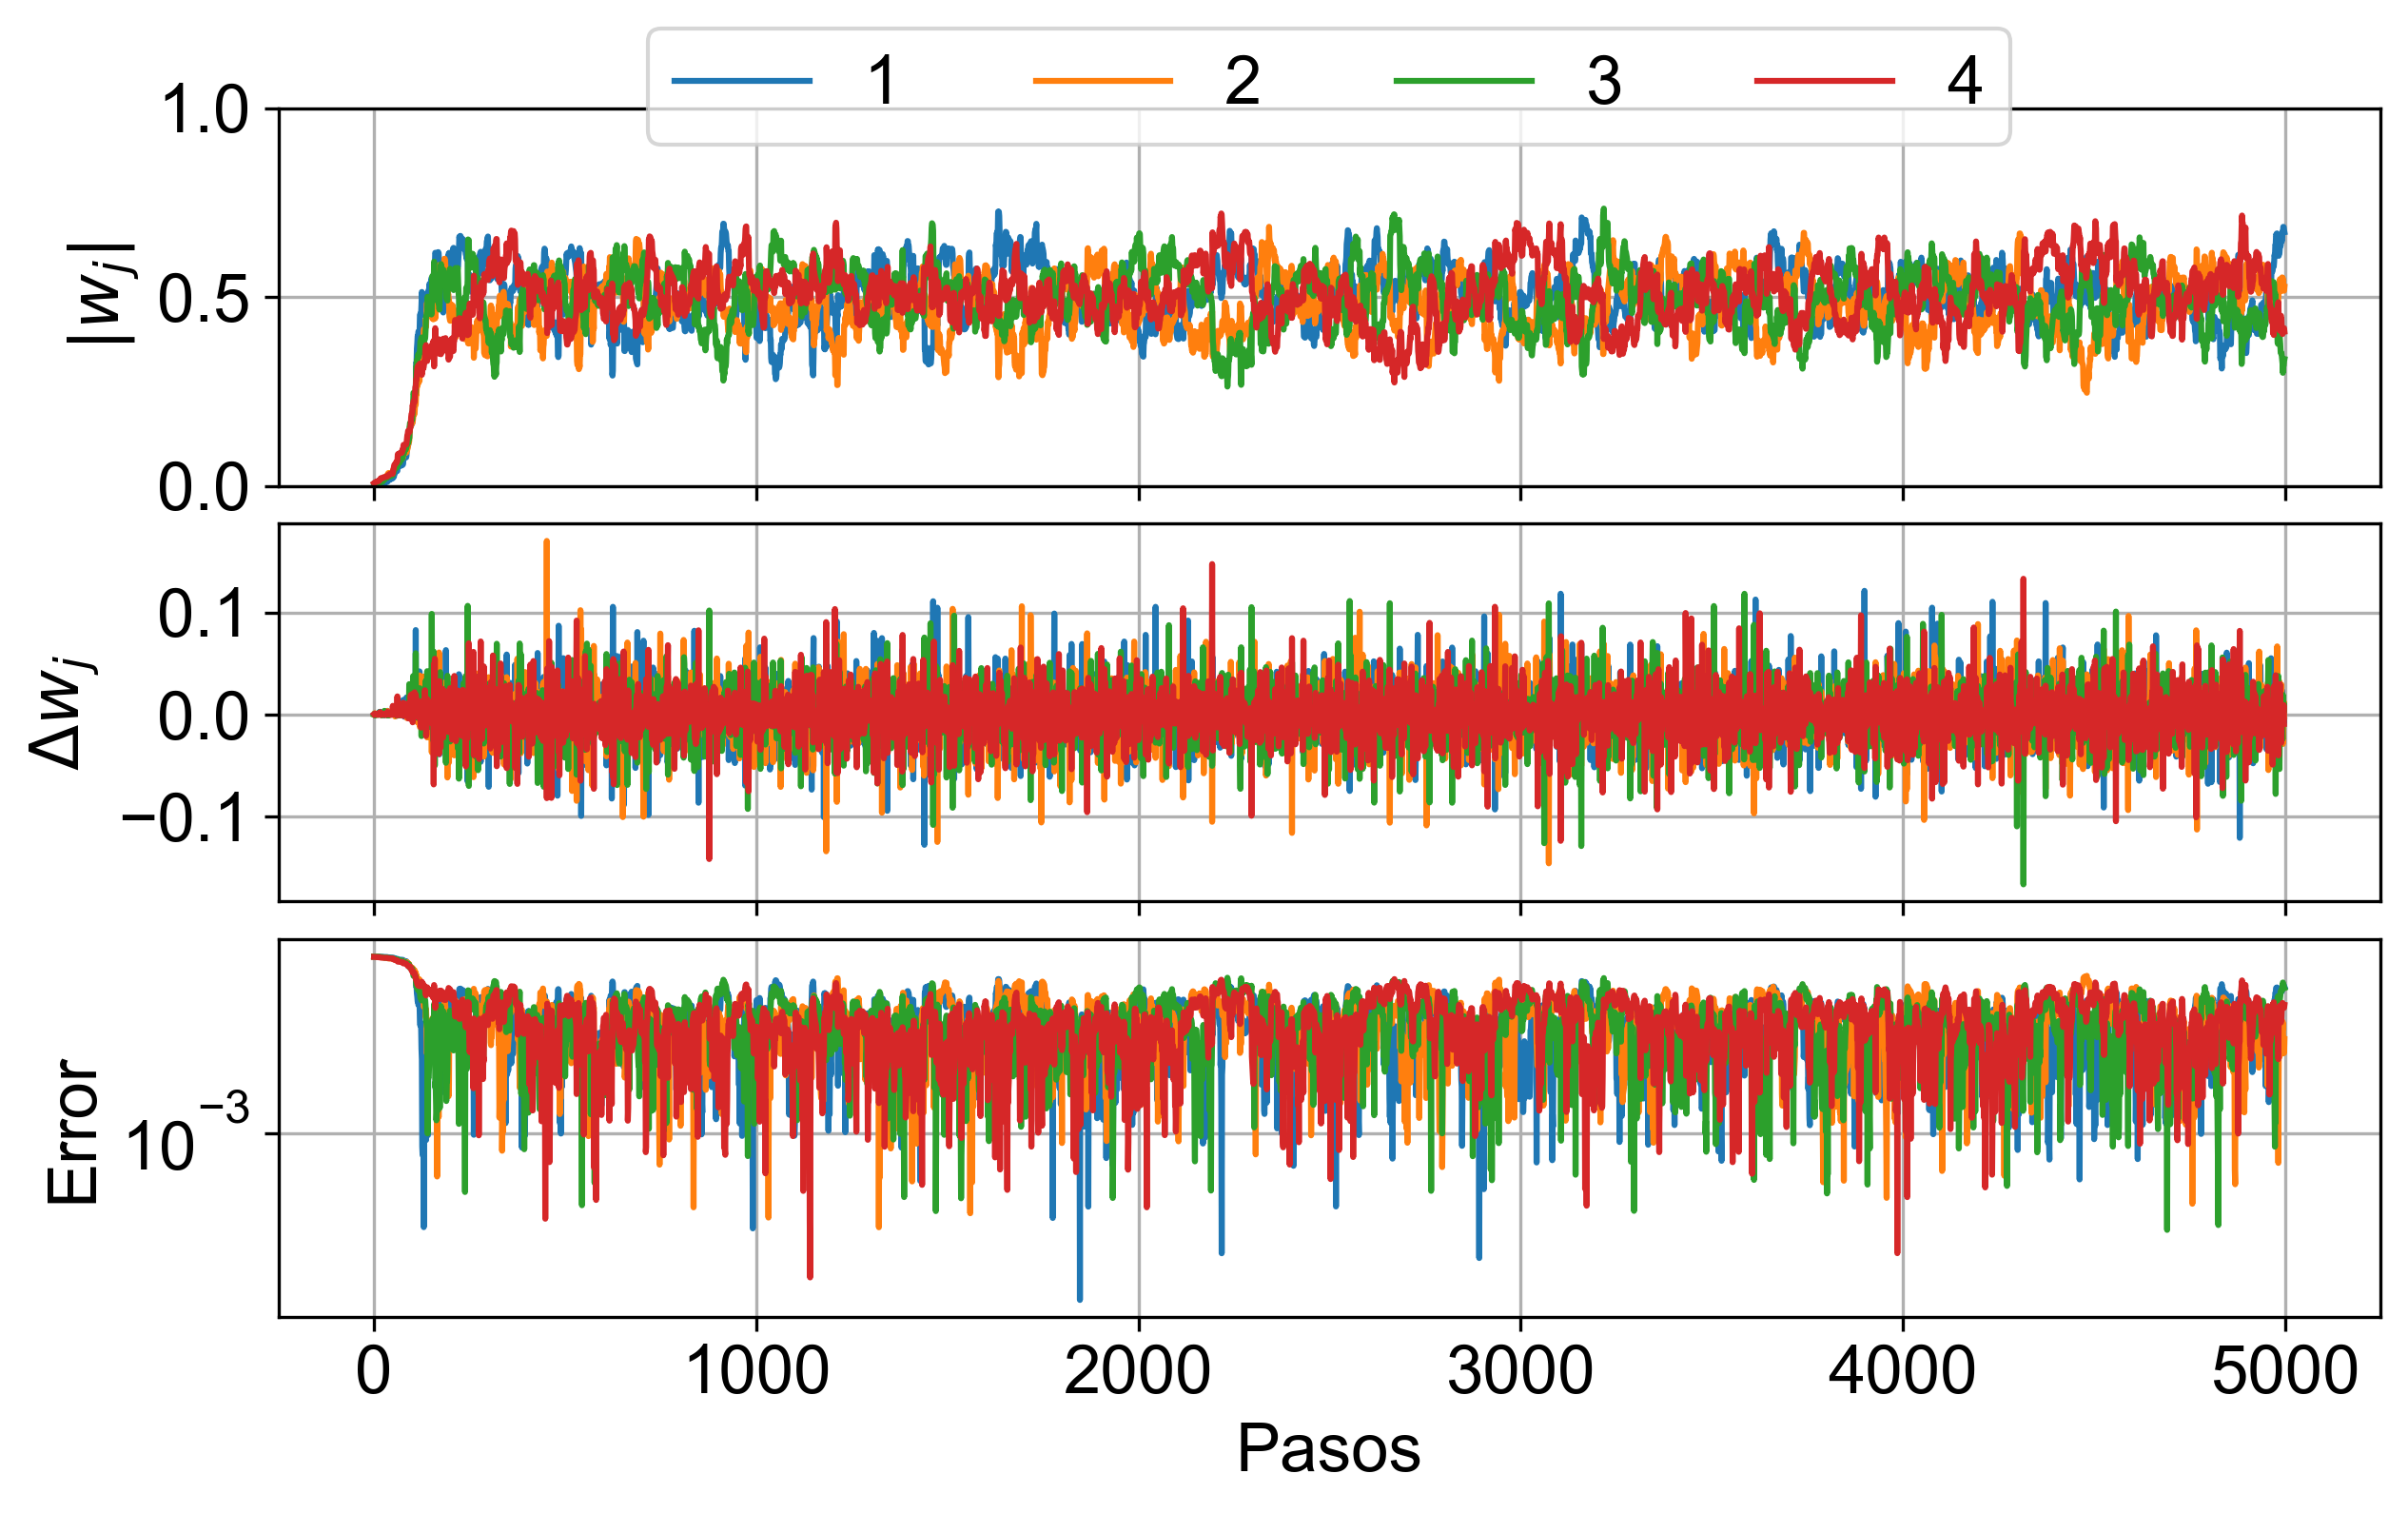
\includegraphics[width=\textwidth]{ej1_fig3.png}
      \caption{\label{fig:ej1_fig3}}
  \end{subfigure}
     \caption{Evolución del módulo de los pesos $w_j$, las modificaciones $\Delta w_j$ y la diferencia entre $w_j$ y $v_j$ durante el entrenamiento de la red neuronal. En \ref{sub@fig:ej1_fig1} se empleó una tasa de aprendizaje de $\eta = 0.001$. En \ref{sub@fig:ej1_fig2} se empleó la misma tasa de aprendizaje pero además se procesaron los datos promediando en cada paso de tiempo sobre los 200 pasos adyacentes. En \ref{sub@fig:ej1_fig3} se empleó una tasa de aprendizaje de $\eta = 0.01$.}
     \label{fig:three graphs}
\end{figure}

\begin{figure}
  \centering
  \begin{subfigure}[b]{0.24\textwidth}
      \centering
      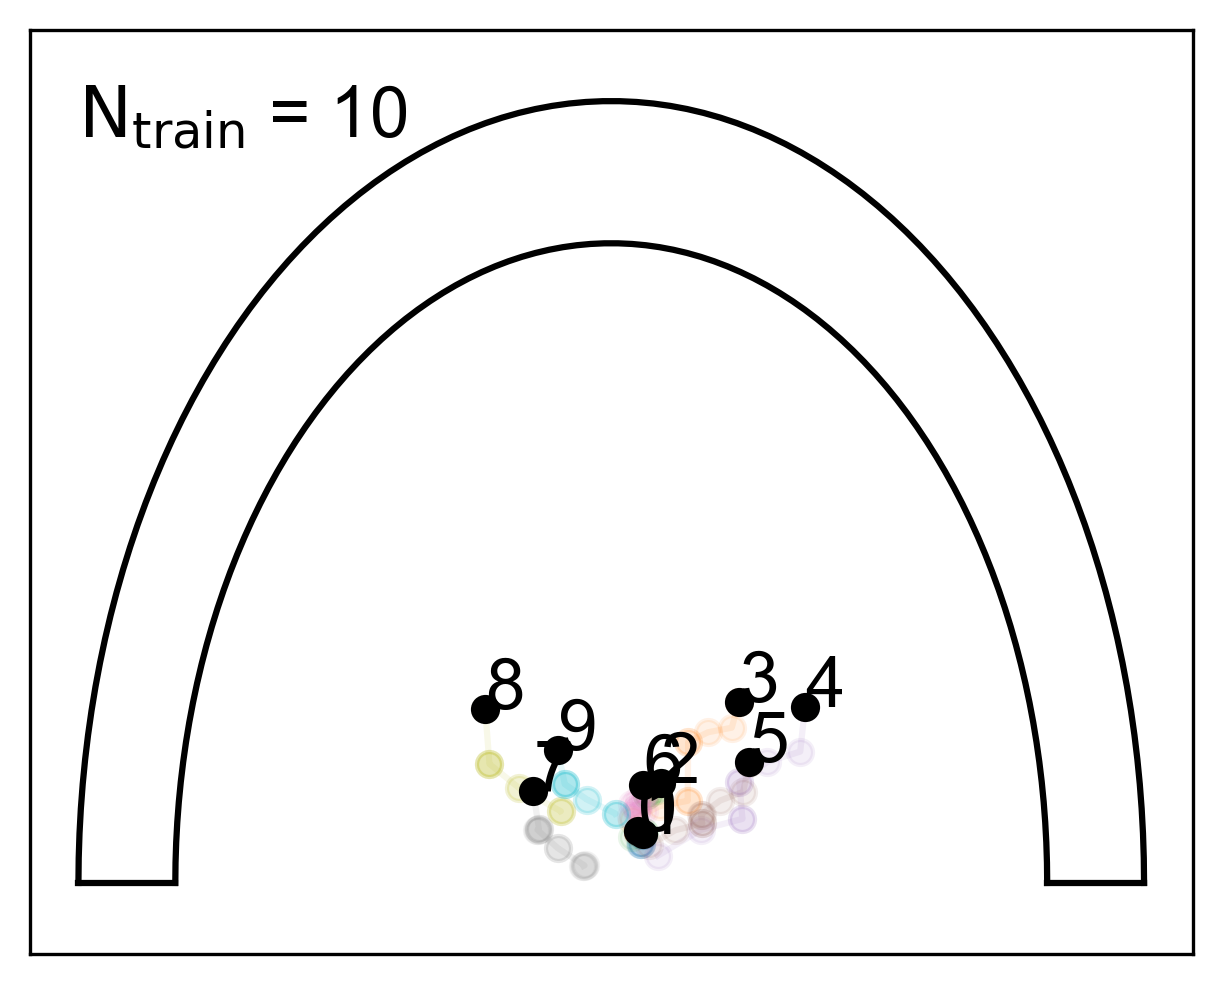
\includegraphics[width=\textwidth]{ej2_fig1_1.png}
      \caption{\label{fig:ej2_fig1_1}}
  \end{subfigure}
  \hfill
  \begin{subfigure}[b]{0.24\textwidth}
      \centering
      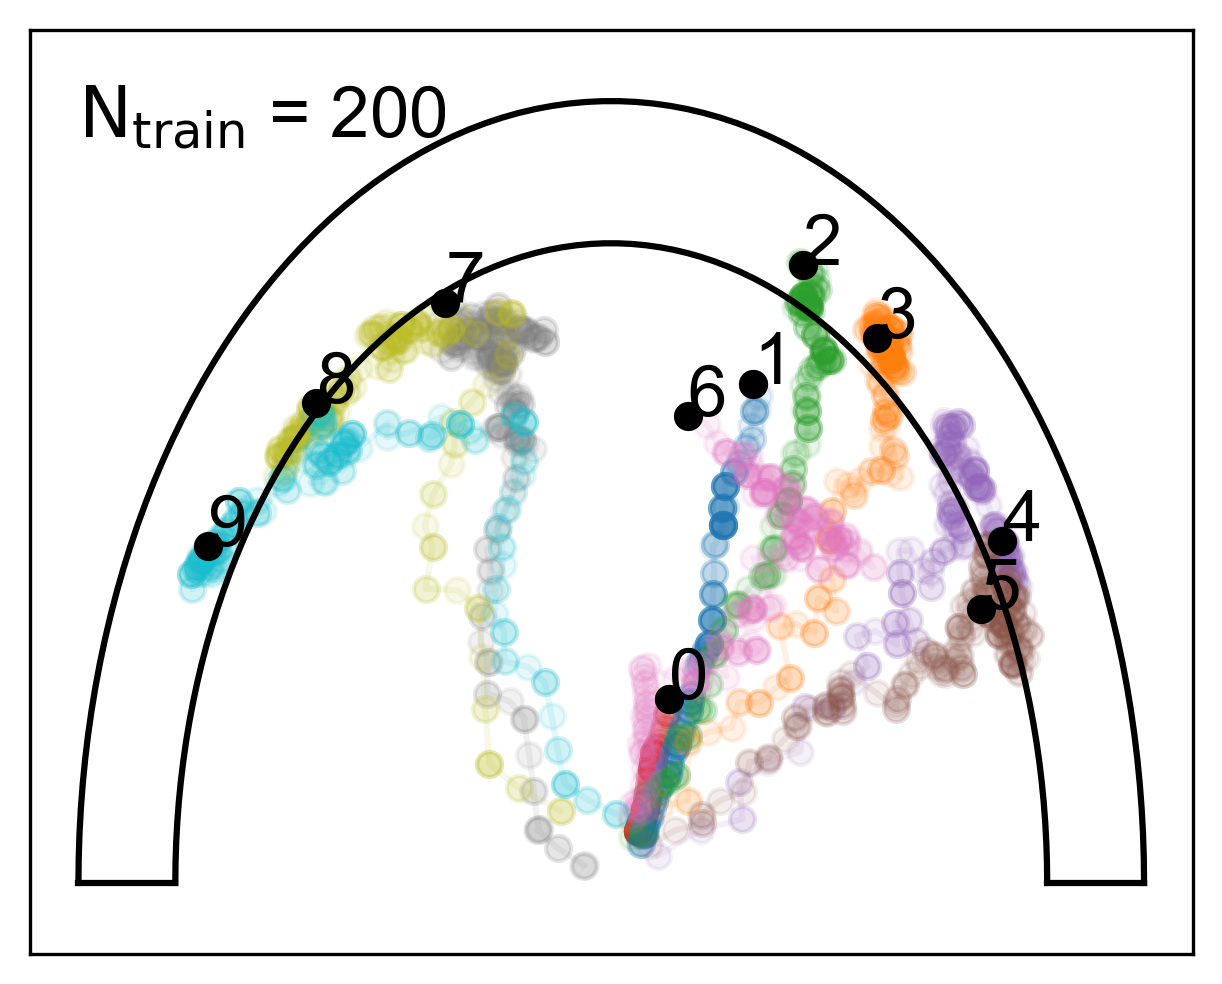
\includegraphics[width=\textwidth]{ej2_fig1_2.png}
      \caption{\label{fig:ej2_fig1_2}}
  \end{subfigure}
  \hfill
  \begin{subfigure}[b]{0.24\textwidth}
      \centering
      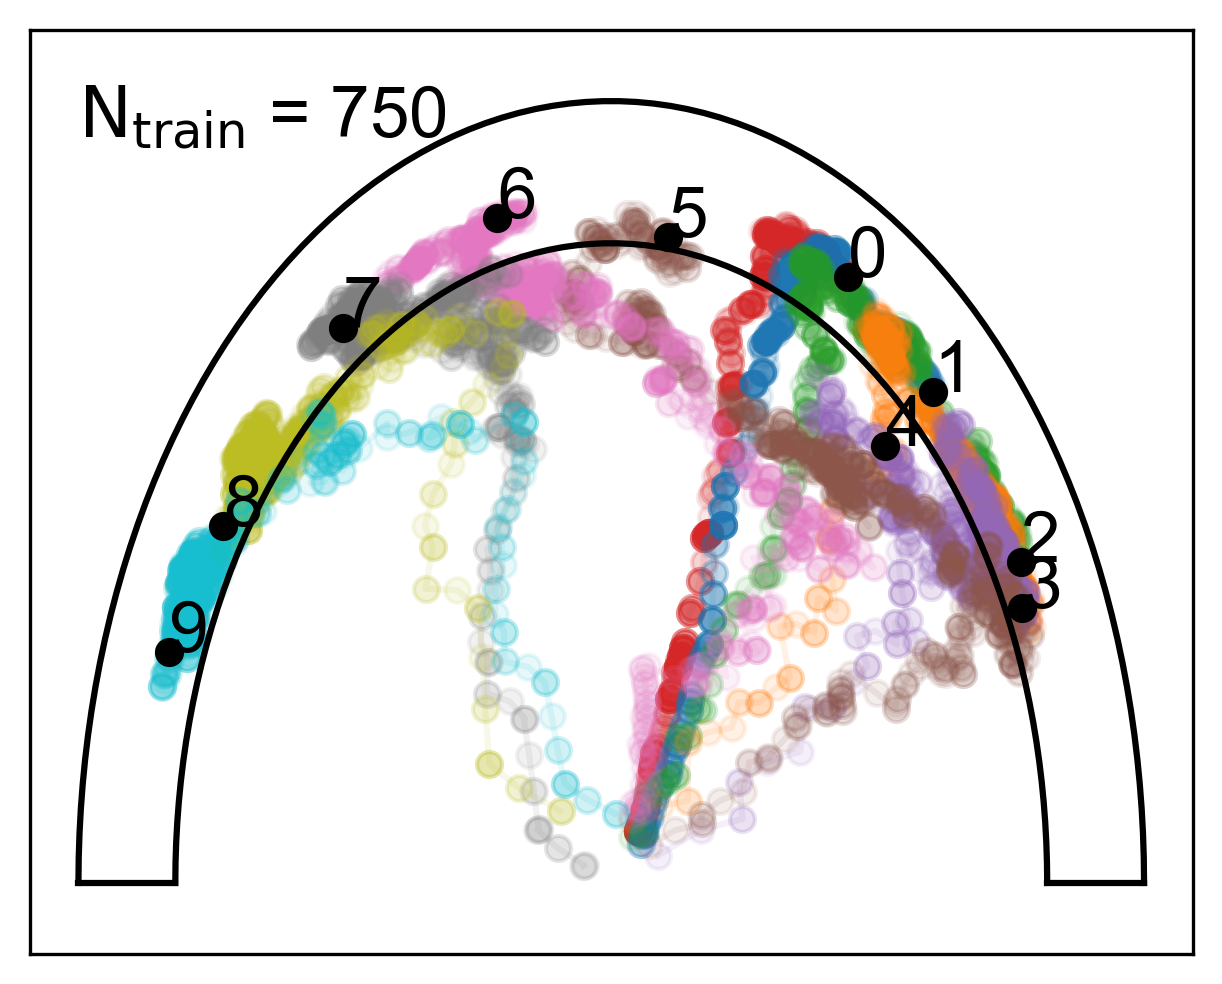
\includegraphics[width=\textwidth]{ej2_fig1_3.png}
      \caption{\label{fig:ej2_fig1_3}}
  \end{subfigure}
  \hfill
  \begin{subfigure}[b]{0.24\textwidth}
      \centering
      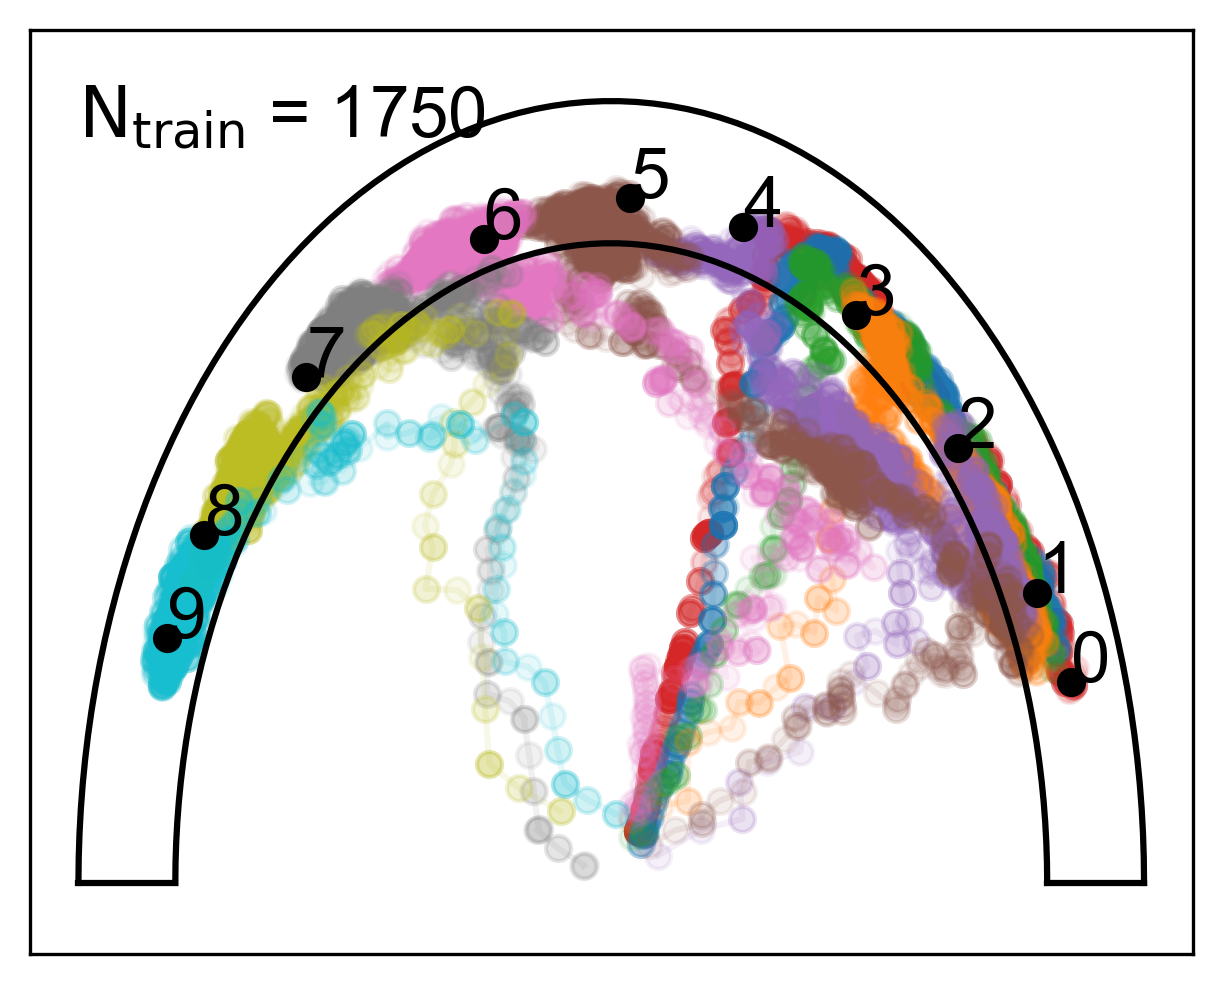
\includegraphics[width=\textwidth]{ej2_fig1_4.png}
      \caption{\label{fig:ej2_fig1_4}}
  \end{subfigure}
  \hfill
  \begin{subfigure}[b]{0.24\textwidth}
      \centering
      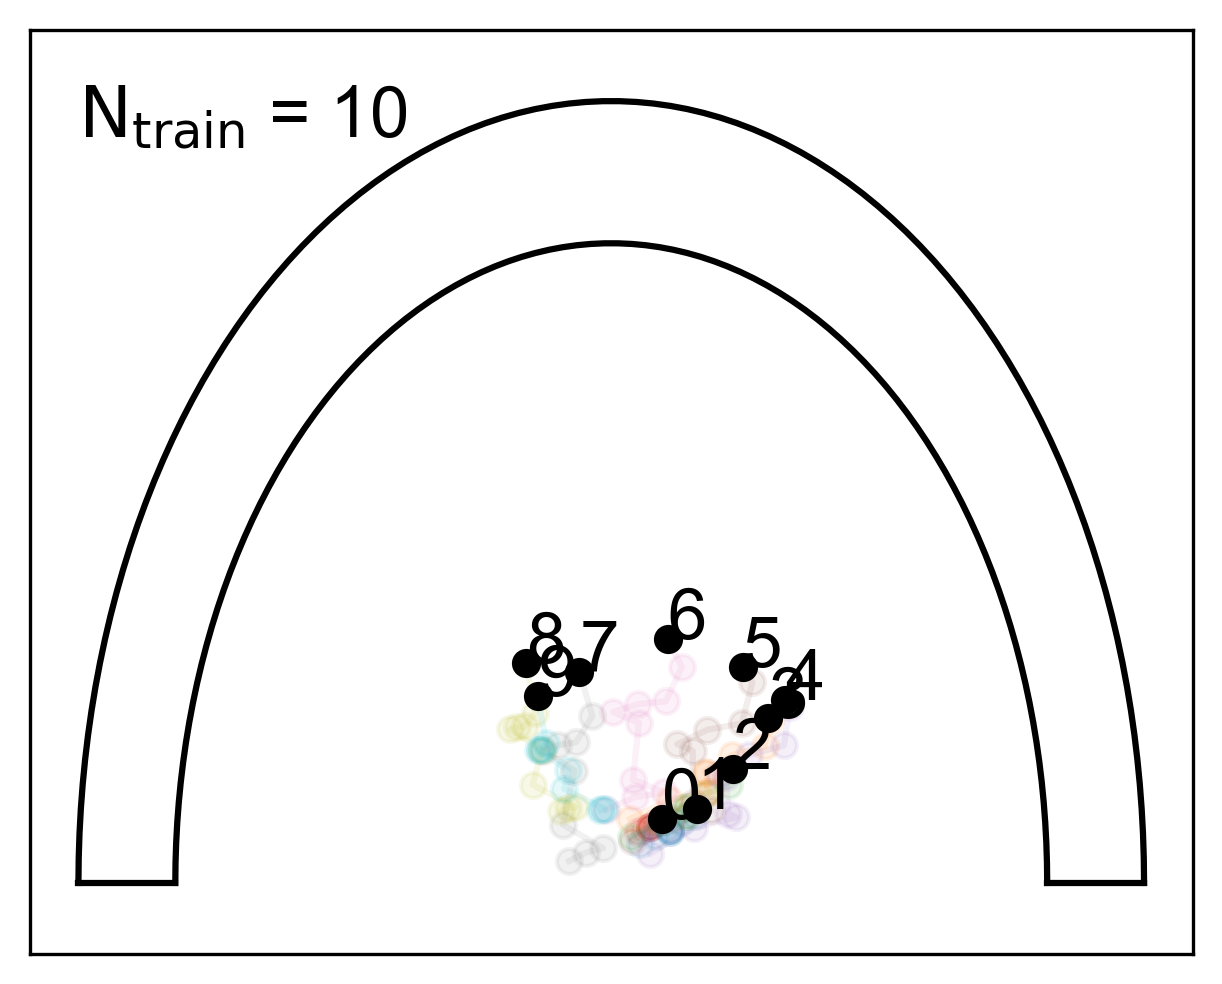
\includegraphics[width=\textwidth]{ej2_fig2_1.png}
      \caption{\label{fig:ej2_fig2_1}}
  \end{subfigure}
  \hfill
  \begin{subfigure}[b]{0.24\textwidth}
      \centering
      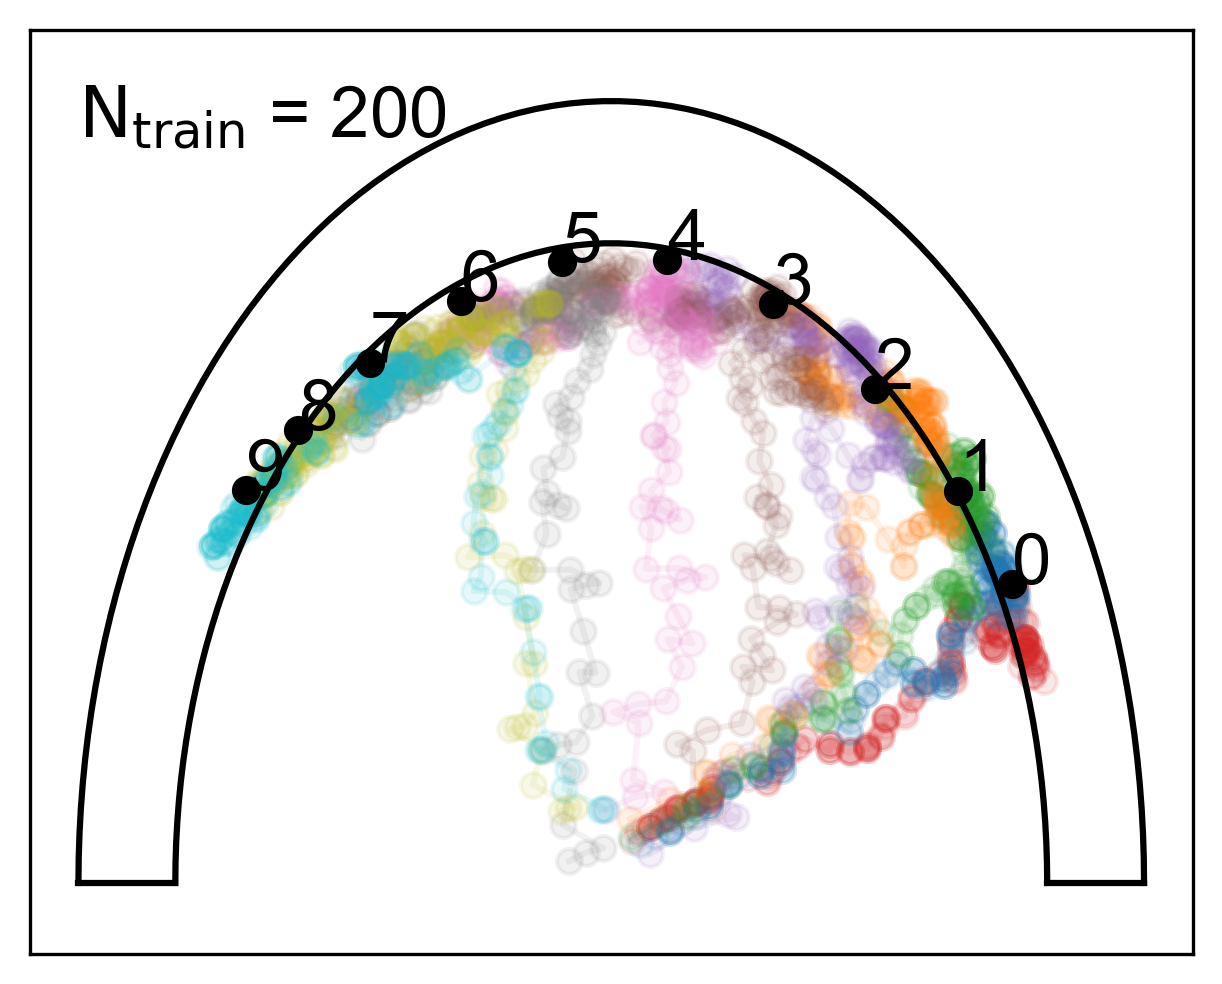
\includegraphics[width=\textwidth]{ej2_fig2_2.png}
      \caption{\label{fig:ej2_fig2_2}}
  \end{subfigure}
  \hfill
  \begin{subfigure}[b]{0.24\textwidth}
      \centering
      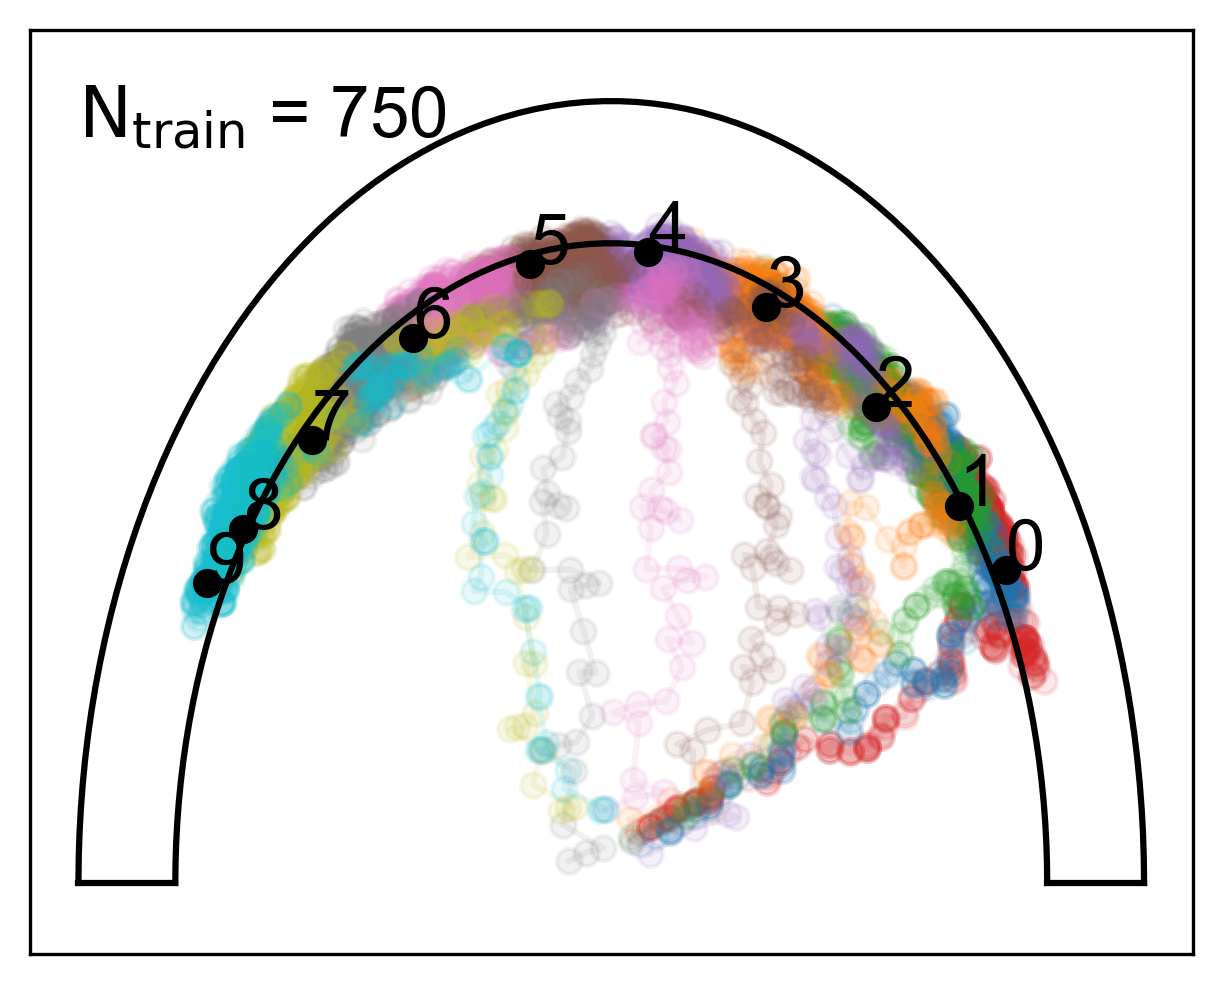
\includegraphics[width=\textwidth]{ej2_fig2_3.png}
      \caption{\label{fig:ej2_fig2_3}}
  \end{subfigure}
  \hfill
  \begin{subfigure}[b]{0.24\textwidth}
      \centering
      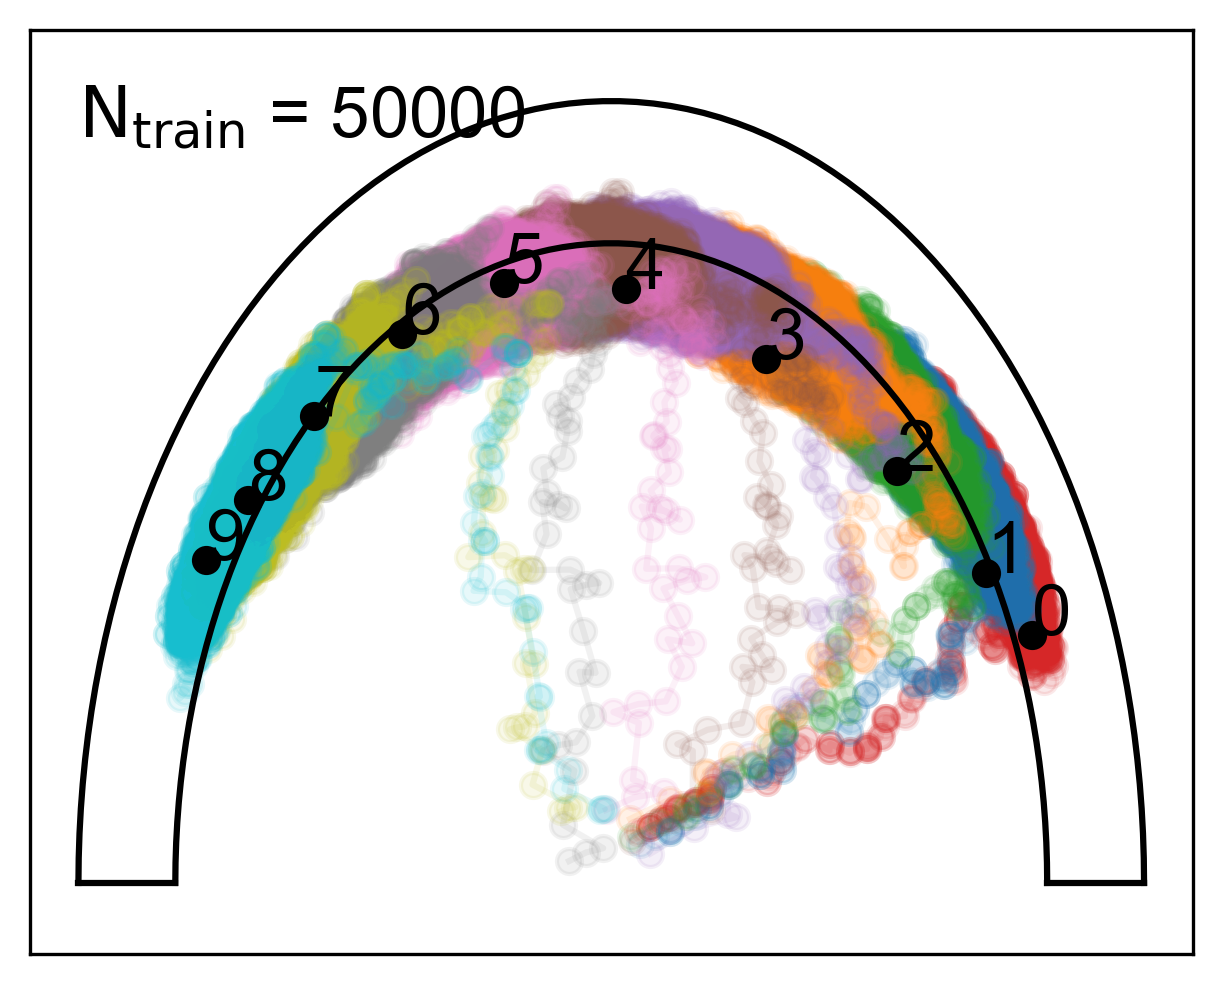
\includegraphics[width=\textwidth]{ej2_fig2_4.png}
      \caption{\label{fig:ej2_fig2_4}}
  \end{subfigure}
  \hfill
  \begin{subfigure}[b]{0.24\textwidth}
      \centering
      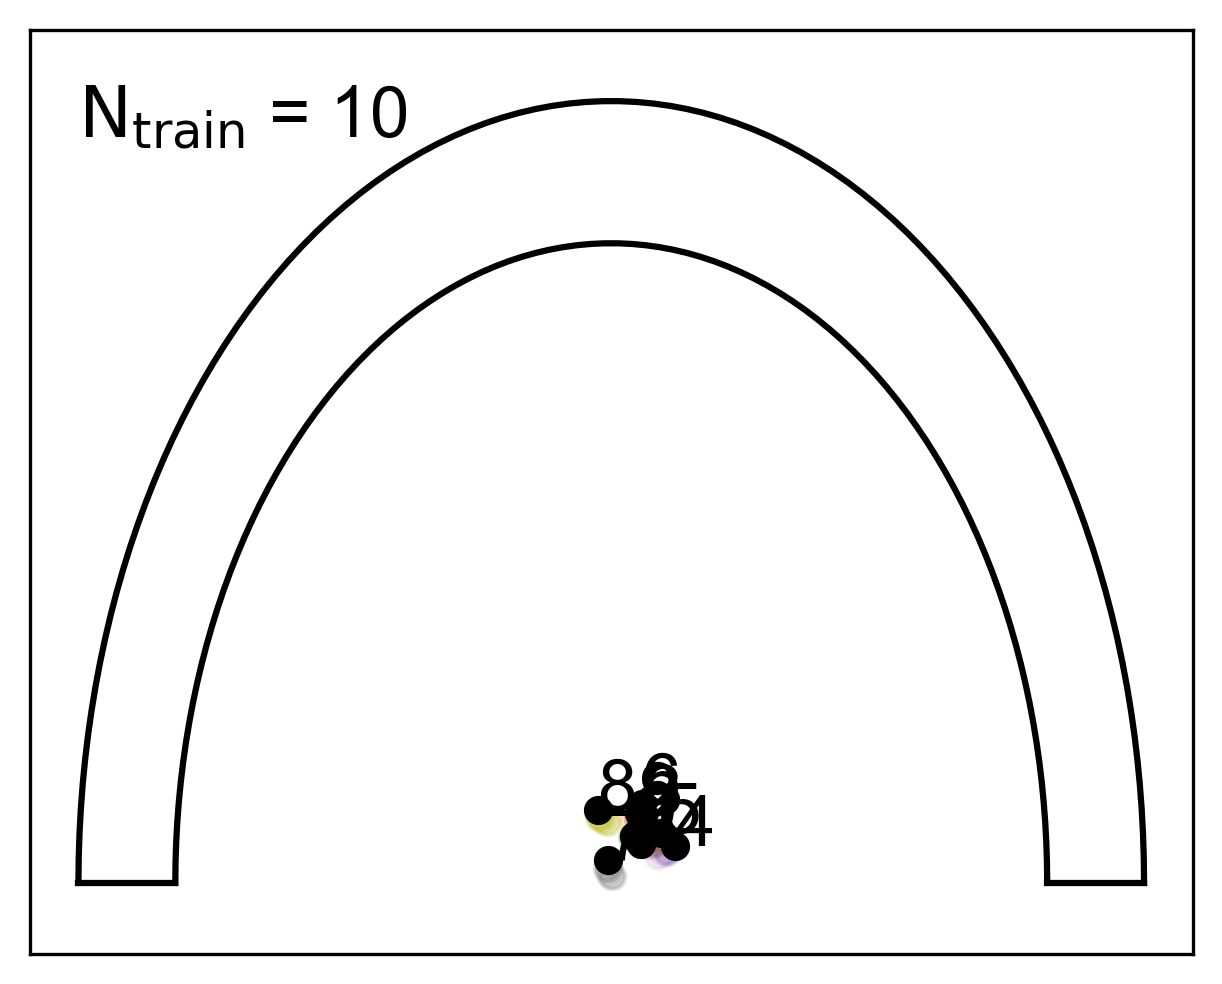
\includegraphics[width=\textwidth]{ej2_fig3_1.png}
      \caption{\label{fig:ej2_fig3_1}}
  \end{subfigure}
  \hfill
  \begin{subfigure}[b]{0.24\textwidth}
      \centering
      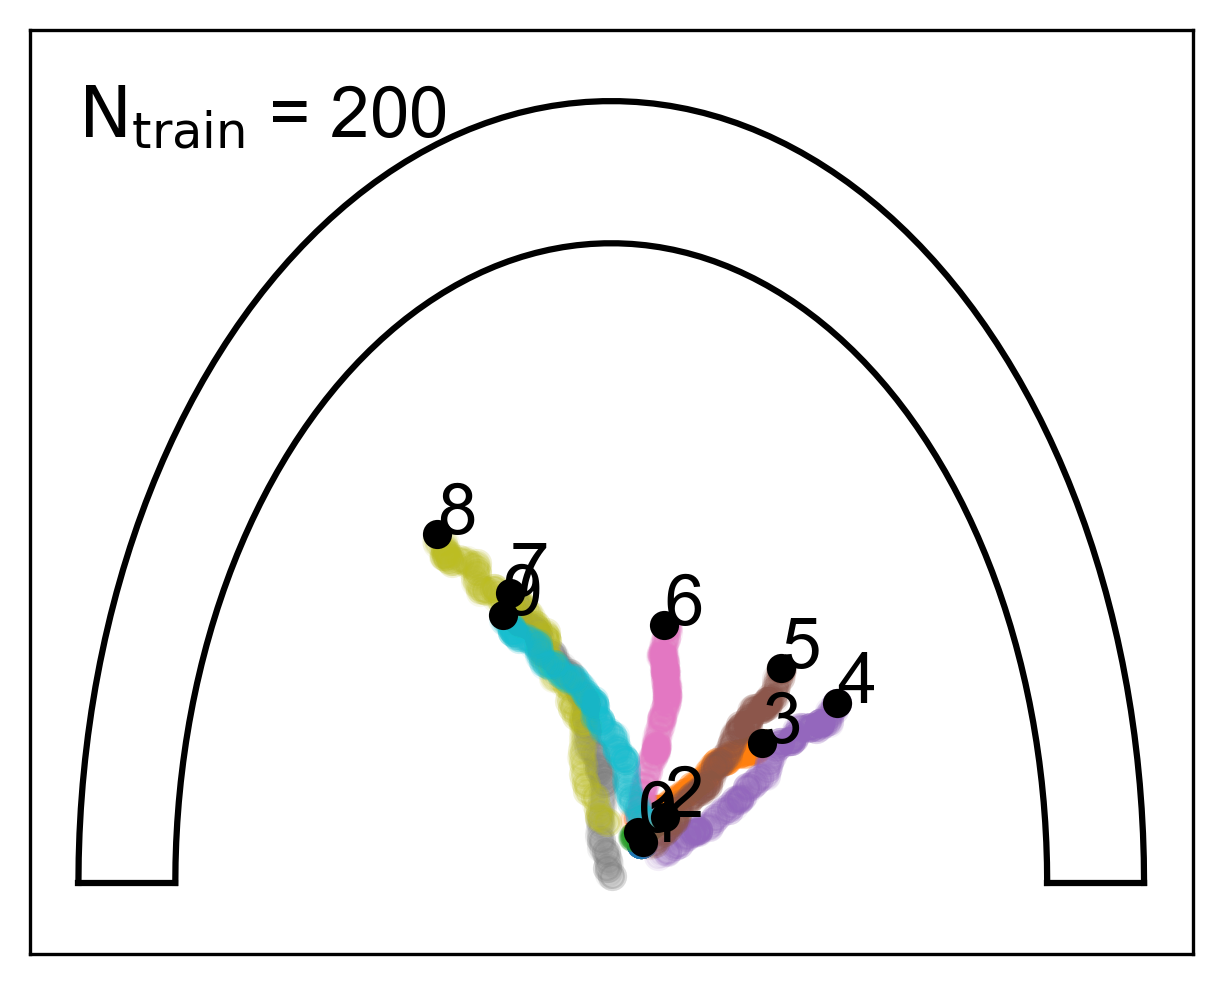
\includegraphics[width=\textwidth]{ej2_fig3_2.png}
      \caption{\label{fig:ej2_fig3_2}}
  \end{subfigure}
  \hfill
  \begin{subfigure}[b]{0.24\textwidth}
      \centering
      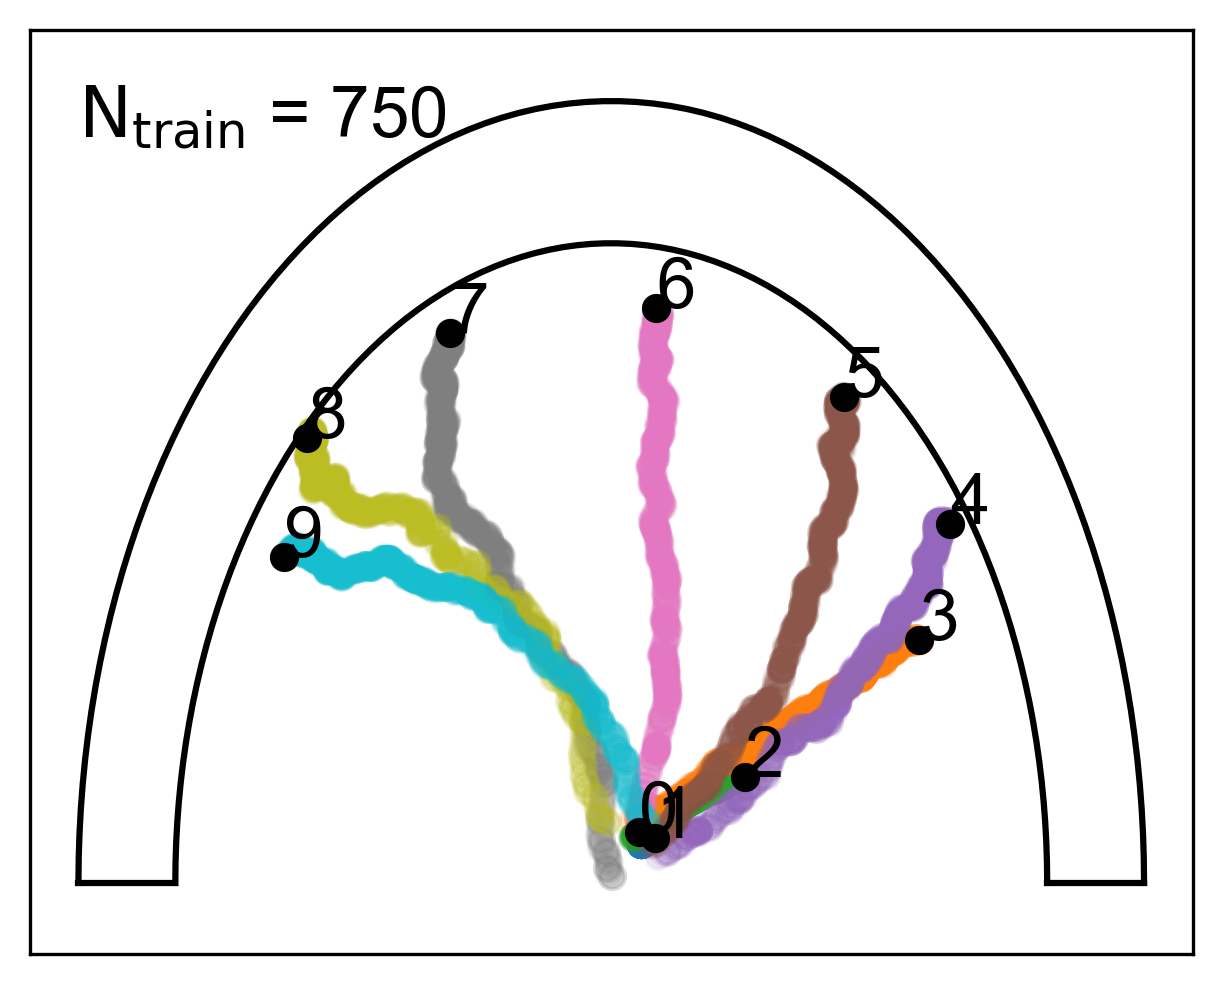
\includegraphics[width=\textwidth]{ej2_fig3_3.png}
      \caption{\label{fig:ej2_fig3_3}}
  \end{subfigure}
  \hfill
  \begin{subfigure}[b]{0.24\textwidth}
      \centering
      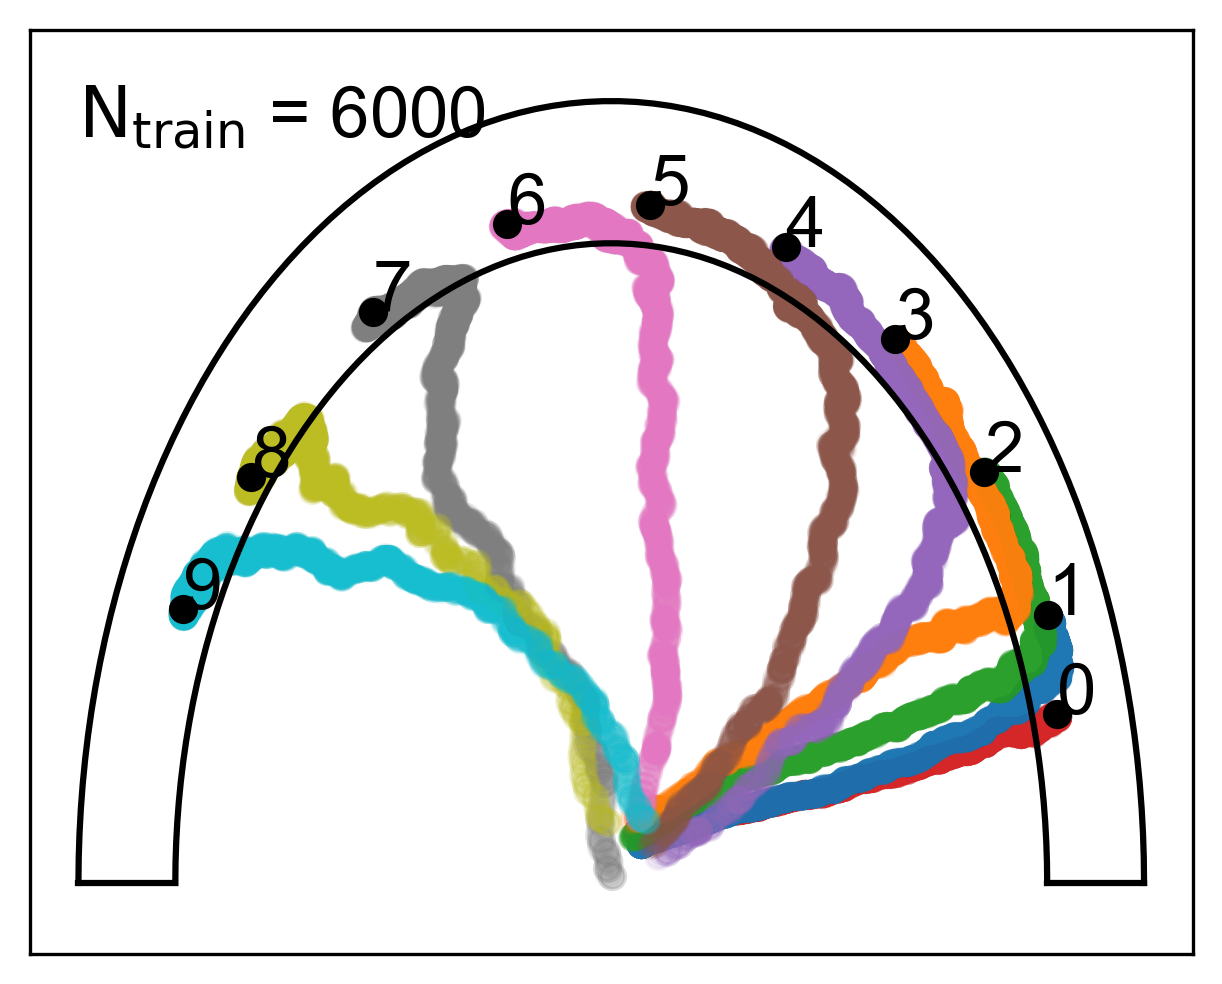
\includegraphics[width=\textwidth]{ej2_fig3_4.png}
      \caption{\label{fig:ej2_fig3_4}}
  \end{subfigure}
     \caption{Evolución de los peso $\vec{w}_i$ con $i = 1$, 2, 3, $\ddots$, 10 en el espacio de los datos de entrada para distintos pasos de entrenamiento $\mathrm{N_{train}}$. Se empleó \ref{sub@fig:ej2_fig1_1}-\ref{sub@fig:ej2_fig1_4} $\eta = 0.1$, $\sigma = 1$, \ref{sub@fig:ej2_fig2_1}-\ref{sub@fig:ej2_fig2_4} $\eta = 0.1$, $\sigma = 2$, \ref{sub@fig:ej2_fig3_1}-\ref{sub@fig:ej2_fig3_4} $\eta = 0.01$, $\sigma = 1$. La región semicircular corresponde a la región donde se encuentran los datos de entrada. En negro se grafica la posición de los pesos finales para cada valor de $\mathrm{N_{train}}$, junto al número correspondiente de neurona. La numeración de las neuronas se realiza en base a que se encuentran dispuestas en una línea. En color se grafican las posiciones previas. No se grafican los ejes por simplicidad.}
     \label{fig:ej2_fig1}
\end{figure}

\newpage

\section*{Apéndice}
A continuación se desarrolla el código empleado durante este trabajo implementado en Python.




\begin{lstlisting}[language=Python]
  #Import libraries
  import numpy as np
  import matplotlib
  import matplotlib.pyplot as plt
  import tensorflow as tf
  
  

\end{lstlisting}

\bibliography{Chehade_practica_5.bib}

\end{document}





